\documentclass{beamer}
\usepackage{times}
\usepackage{amsmath,amsthm, amssymb}

\usepackage[T1]{fontenc}
\usepackage{lmodern}

\usepackage{graphicx}
\usepackage{caption}
\usepackage{booktabs}
\usepackage{siunitx}
\usepackage{tikz}
\usepackage{subcaption}
\usepackage{pgfplots}
\pgfplotsset{compat=1.17}
\newcommand{\blu}{\color{blue}}
\usepackage{DejaVuSans}
\usepackage[backend=biber,style=ieee]{biblatex}

\addbibresource{poster.bib}

\boldmath
\usetheme{gemini}
\usecolortheme{purple}
\usepackage[orientation=portrait,size=a0,scale=1.2]{beamerposter}

\newlength{\sepwidthA} % Seperation distance between comulumns type A
\newlength{\colwidthA} % collumn width type A
\setlength{\sepwidthA}{0.01\paperwidth}
\setlength{\colwidthA}{0.95\paperwidth}

\newcommand{\separatorcolumnA}{\begin{column}{\sepwidthA}\end{column}}

% Second column environment.
\newlength{\sepwidthB}
\newlength{\colwidthB}
\setlength{\sepwidthB}{0.01\paperwidth}
\setlength{\colwidthB}{0.45\paperwidth}

\newcommand{\separatorcolumnB}{\begin{column}{\sepwidthB}\end{column}}

\title[Beamer Poster]{\huge{Separation of primary particles\\in a LHCb-like EM calorimeter}}
\author[ccatamorenos@gmail.com]{
Author: Cindy Catalina Moreno Sarria\\
Directors: Ph.D. Carlos Eduardo Sandoval Usme\\
Ph.D. Diego Alejandro Milanés Carreño
}
\institute[UNAL]
{
FENYX\\
Programa de Pregrado en Física
}
\date{}

% \logo{
\includegraphics[height=7.5cm]{assets/Logo_UNAL.png}}

\footercontent{
\href{mailto:ccatamorenos@gmail.com}{ccatamorenos@gmail.com} % this is a clickable link
}

\begin{document}
\begin{frame}{}

  \begin{tikzpicture}[remember picture,overlay,line width=\arrayrulewidth] % gradient header bar
      % UQ Reverse Logo
      \node [anchor=north west, inner sep=3cm] at ([xshift=0cm,yshift=-1cm]current page.north west)
      {
\includegraphics[height=8.0cm]{assets/Logo_UNAL.png}};
    \end{tikzpicture}

    \begin{columns}[t]
      \separatorcolumnA
      \begin{column}{\colwidthA}

        \begin{block}{Abstract}
          \begin{figure}
            {\small Five different multidimensional classifiers (MultinomialNB,
            BernoulliNB, Perceptron, SGDClassifier and
            PassiveAggressiveClassifier) were used to test the capability of
            primary particle discrimination in an LHCb-like electromagnetic
            calorimeter using sampling data from Geant4 simulation. The
            classifiers were supposed to differentiate between photons,
            electrons and neutral pions, given the number of electrons and
            photons created in the scintillator and lead plates in the
            calorimeter. They however did not show a good performance in this
            task, having a accuracy of 0.45 for MultinomialNB, 0.55 for
            BernoulliNB, 0.33 for Perceptron, 0.33 for SGDClassifier and 0.33
            for PassiveAggressiveClassifier.}
          \end{figure}
        \end{block}

      \end{column}

      \separatorcolumnA
    \end{columns}

    \begin{columns}

      \begin{column}[T]{\colwidthB}

        \begin{block}{Introduction}

          The identification of high energetic \(\pi^0\) events in the
          electromagnetic calorimeter is not optimal. The neutral pion decays
          into two quite parallel photons, that can be misinterpreted as a
          single photon with high energy. An alternative to the primary
          particle identification is the implementation of machine learning
          algorithms\cite{Boldyrev_2020}.

        \end{block}

        \begin{block}{Methods}

          The study was divided in two parts, a simulation of an
          electromagnetic calorimeter in Geant4, inspired in the design of ECAL
          in the LHCb experiment. and a machine learning implementation for
          multivariable classification.

          \textbf{Simulation}

          The calorimeter is composed by a mesh of \(6\times4\) modules. Each
          module is a combination of thin layers of scintillator and lead.

          \begin{figure}[htb]
            \centering

            \subfloat[Complete calorimeter.]{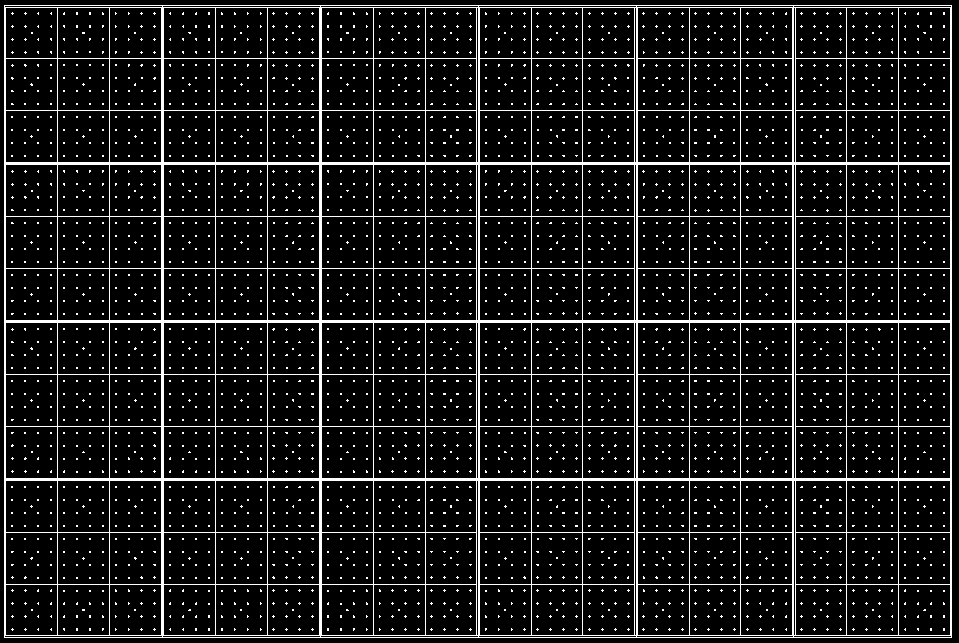
\includegraphics[width=0.40\textwidth]{assets/ecal-inner-section-cropped-geometry-2.png}\label{fig:cropped-geometry-2}}\hspace{2em}
            \subfloat[Module.]{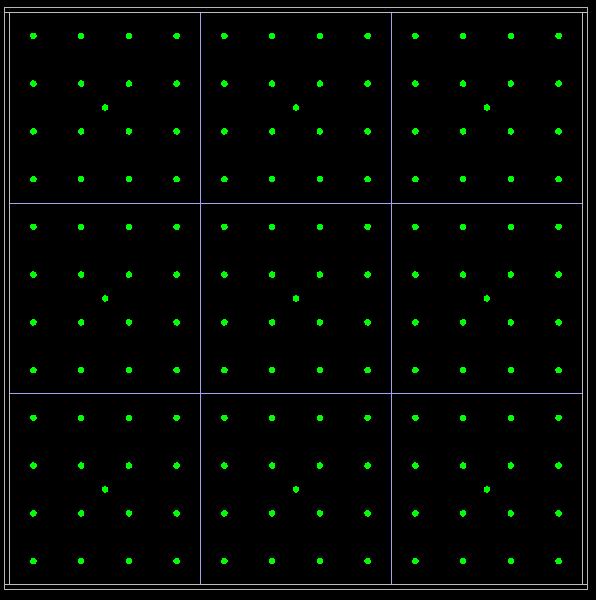
\includegraphics[width=0.40\textwidth]{assets/Mesh.png}\label{fig:cropped-geometry-1}}

            \caption{Front view of the detector.}\label{fig:cropped-geometry}

          \end{figure}

          \textbf{Machine Learning implementation}

          For the machine learning implementation, the classifiers
          MultinomialNB, BernoulliNB, Perceptron, SGDClassifier and
          PassiveAggressiveClassifier were used to separate the primary
          particles.

        \end{block}

      \end{column}
      \separatorcolumnB

      \begin{column}[T]{\colwidthB}

        \begin{block}{Results}

          Some classifiers do not show good performance in the differentiation
          task, specially the linear classifiers. It could be due to the amount
          of variables that are considered in the input, the low discrepancy
          between theirs distributions and the no linearity between them. The
          best separation was found for BernoulliNB.

          \begin{table}[hbt]
            \centering
            \begin{tabular}{c c}
              \textbf{Classifier} & \textbf{Result}\\
              \toprule
              MultinomialNB & 0.45\\
              \midrule
              BernoulliNB & 0.55\\
              \midrule
              Perceptron & 0.33\\
              \midrule
              SGDClassifier & 0.33\\
              \midrule
              PassiveAggressiveClassifier & 0.33\\
              \bottomrule
            \end{tabular}
            \caption{Accuracy of the machine learning methods.}\label{tb:machine-learning-results}
          \end{table}

        \end{block}

        \begin{figure}[htb]
          \centering

          \subfloat[]{\includegraphics[width=0.49\textwidth]{assets/scores1.pdf}\label{fig:cropped-geometry-3}}
          \subfloat[]{\includegraphics[width=0.49\textwidth]{assets/scores2.pdf}\label{fig:cropped-geometry-4}}

          \caption{Accuracy of the machine learning methods during training.}\label{fig:cropped-geometry-g}

        \end{figure}

        \begin{block}{References}

          \nocite{*}
          \printbibliography
        \end{block}

      \end{column}

    \end{columns}


\end{frame}
\end{document}
